\documentclass{beamer}\usepackage[]{graphicx}\usepackage[]{color}
%% maxwidth is the original width if it is less than linewidth
%% otherwise use linewidth (to make sure the graphics do not exceed the margin)
\makeatletter
\def\maxwidth{ %
  \ifdim\Gin@nat@width>\linewidth
    \linewidth
  \else
    \Gin@nat@width
  \fi
}
\makeatother

\definecolor{fgcolor}{rgb}{0.345, 0.345, 0.345}
\newcommand{\hlnum}[1]{\textcolor[rgb]{0.686,0.059,0.569}{#1}}%
\newcommand{\hlstr}[1]{\textcolor[rgb]{0.192,0.494,0.8}{#1}}%
\newcommand{\hlcom}[1]{\textcolor[rgb]{0.678,0.584,0.686}{\textit{#1}}}%
\newcommand{\hlopt}[1]{\textcolor[rgb]{0,0,0}{#1}}%
\newcommand{\hlstd}[1]{\textcolor[rgb]{0.345,0.345,0.345}{#1}}%
\newcommand{\hlkwa}[1]{\textcolor[rgb]{0.161,0.373,0.58}{\textbf{#1}}}%
\newcommand{\hlkwb}[1]{\textcolor[rgb]{0.69,0.353,0.396}{#1}}%
\newcommand{\hlkwc}[1]{\textcolor[rgb]{0.333,0.667,0.333}{#1}}%
\newcommand{\hlkwd}[1]{\textcolor[rgb]{0.737,0.353,0.396}{\textbf{#1}}}%
\let\hlipl\hlkwb

\usepackage{framed}
\makeatletter
\newenvironment{kframe}{%
 \def\at@end@of@kframe{}%
 \ifinner\ifhmode%
  \def\at@end@of@kframe{\end{minipage}}%
  \begin{minipage}{\columnwidth}%
 \fi\fi%
 \def\FrameCommand##1{\hskip\@totalleftmargin \hskip-\fboxsep
 \colorbox{shadecolor}{##1}\hskip-\fboxsep
     % There is no \\@totalrightmargin, so:
     \hskip-\linewidth \hskip-\@totalleftmargin \hskip\columnwidth}%
 \MakeFramed {\advance\hsize-\width
   \@totalleftmargin\z@ \linewidth\hsize
   \@setminipage}}%
 {\par\unskip\endMakeFramed%
 \at@end@of@kframe}
\makeatother

\definecolor{shadecolor}{rgb}{.97, .97, .97}
\definecolor{messagecolor}{rgb}{0, 0, 0}
\definecolor{warningcolor}{rgb}{1, 0, 1}
\definecolor{errorcolor}{rgb}{1, 0, 0}
\newenvironment{knitrout}{}{} % an empty environment to be redefined in TeX

\usepackage{alltt}
\usepackage{../371g-slides}
% Uncomment these lines to print notes pages
% \pgfpagesuselayout{4 on 1}[letterpaper,border shrink=5mm,landscape]
% \setbeameroption{show only notes}
\title{Probability Review 3}
\subtitle{Lecture 4}
\author{STA 371G}
\IfFileExists{upquote.sty}{\usepackage{upquote}}{}
\begin{document}
  
  

  \frame{\maketitle}

  % Show outline at beginning of each section
  \AtBeginSection[]{ 
    \begin{frame}<beamer>
      \tableofcontents[currentsection]
    \end{frame}
  }

  %%%%%%% Slides start here %%%%%%%

  \begin{darkframes}
    \begin{frame}
      \begin{itemize}
        \item Starting tonight: Weekly R help session in the ModLab, 6:30-7:30 PM
      \end{itemize}
    \end{frame}

    \begin{frame}{Who are these people?}
      \begin{columns}[onlytextwidth]
        \column{.3\textwidth}
          \begin{center}
            
\includegraphics[width=0.8in]{zack} \\
            Zack
          \end{center}
        \column{.3\textwidth}
          \begin{center}
            
\includegraphics[width=0.8in]{kelly} \\
            Kelly
          \end{center}
        \column{.3\textwidth}
          \begin{center}
            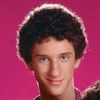
\includegraphics[width=0.8in]{screech} \\
            Screech
          \end{center}
      \end{columns}
      \smallskip
      \begin{columns}[onlytextwidth]
        \column{.3\textwidth}
          \begin{center}
            
\includegraphics[width=0.8in]{slater} \\
            Slater
          \end{center}
        \column{.3\textwidth}
          \begin{center}
            
\includegraphics[width=0.8in]{jessie} \\
            Jessie
          \end{center}
        \column{.3\textwidth}
          \begin{center}
            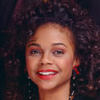
\includegraphics[width=0.8in]{lisa} \\
            Lisa
          \end{center}
      \end{columns}
    \end{frame}

    \begin{frame}{Some events}
      \begin{columns}[onlytextwidth]
        \column{.2\textwidth}
          
\includegraphics[width=0.45in]{zack} \\
          
\includegraphics[width=0.45in]{kelly} \\
          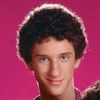
\includegraphics[width=0.45in]{screech} \\
          
\includegraphics[width=0.45in]{slater} \\
          
\includegraphics[width=0.45in]{jessie} \\
          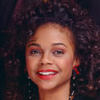
\includegraphics[width=0.45in]{lisa} \\
        \column{.8\textwidth}
          Suppose we pick a \emph{Saved by the Bell} character at random. Each of these are events:
          \begin{itemize}[<+->]
            \item $M = $ we select a male character
            \item $L = $ we select someone with lush hair, where ``lush'' means ``long curly hair'' (mullet included!)
            \item $M|L = $ we select a male \emph{from among the lush-haired characters}
            \item $L|M = $ we select a lush-haired character \emph{from among the male characters}
          \end{itemize}
          \pause
          $P(M) = \pause 3/6$ \qquad $P(L) = \pause 3/6$ \\
          $P(M|L) = \pause 1/3$ \qquad $P(L|M) = \pause 1/3$ \\
      \end{columns}

    \end{frame}

    \begin{frame}{Joint probability}
      \begin{columns}[onlytextwidth]
        \column{.2\textwidth}
          
\includegraphics[width=0.45in]{zack} \\
          
\includegraphics[width=0.45in]{kelly} \\
          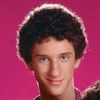
\includegraphics[width=0.45in]{screech} \\
          
\includegraphics[width=0.45in]{slater} \\
          
\includegraphics[width=0.45in]{jessie} \\
          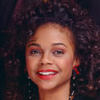
\includegraphics[width=0.45in]{lisa} \\
      \column{.8\textwidth}
        \begin{align*}
          \onslide<1->{P(\text{$M$ and $L$}) &= \text{probability of selecting a lush-haired male} \\}
          \onslide<2->{ &= 1/6 \\} 
          \onslide<3->{ &= P(M)P(L|M) = \frac 3 6 \cdot \frac 1 3 \\}
          \onslide<3->{ &= P(L)P(M|L) = \frac 3 6 \cdot \frac 1 3 \\}
          \onslide<4->{ &\neq P(M)P(L)}
        \end{align*}
      \end{columns}
    \end{frame}

    \begin{frame}{One or the other}
      \begin{columns}[onlytextwidth]
        \column{.2\textwidth}
          
\includegraphics[width=0.45in]{zack} \\
          
\includegraphics[width=0.45in]{kelly} \\
          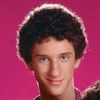
\includegraphics[width=0.45in]{screech} \\
          
\includegraphics[width=0.45in]{slater} \\
          
\includegraphics[width=0.45in]{jessie} \\
          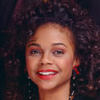
\includegraphics[width=0.45in]{lisa} \\
        \column{.8\textwidth}
          \begin{align*}
            \onslide<1->{P(\text{$M$ or $L$}) &= \text{probability of selecting a lush-haired} \\ & \qquad\text{character, a male character, or both}\\}
            \onslide<2->{ &= 5/6 \\}
            \onslide<3->{ &= P(M) + P(L) - P(\text{$M$ and $L$}) \\ &= 3/6 + 3/6 - 1/6 \\}
          \end{align*}
          \pause
          We have to subtract off $P(\text{$M$ and $L$})$ because otherwise we are double-counting Slater!
      \end{columns}
    \end{frame}

    \begin{frame}{Conditional probability}
      \begin{center}
        When we say $P(A|B)$, what we mean is:
        \bigskip
        ``In a world where we know B has already happened, how likely is it that A also happened?''
      \end{center}
    \end{frame}
    
    \begin{frame}
      \note{Imagine you are living with a partner---your husband/wife/boyfriend/girlfriend---and you come home one day to find underwear of unknown origin on your bedroom dresser!}
      \fullpagepicture{dresser}
    \end{frame}

    \begin{frame}
      \note{What do you do---besides this?!}
      \fullpagepicture{reaction}
    \end{frame}

    \begin{frame}
      \begin{center}
        Now that you’ve found a strange pair of underwear in your dresser, what is the probability that your partner is cheating on you?
        \bigskip
        \[ P(\text{partner is cheating} \mid \text{underwear found}) \]
        \pause\bigskip
        It's hard to know how to estimate this directly!
      \end{center}
    \end{frame}

    \begin{frame}
      Let's come up with estimates for the following:
      \begin{itemize}[<+->]
        \item $P(\text{underwear found} \mid \text{partner is cheating})$
        \item $P(\text{underwear found} \mid \text{partner is not cheating})$
        \item $P(\text{partner is cheating})$ (before we found the underwear!)
      \end{itemize}
    \end{frame}

    \begin{frame}{Bayes' Rule}
      \note{Do the calculation here using the estimates students came up with in the previous slide.}
      \begin{center}
        Bayes' Rule lets us reverse the conditional probabilities!
        
        \bigskip
        
        $U=$ underwear found, $C=$ partner is cheating
      \end{center}

      \[
        P(C|U) = \frac{P(U|C)P(C)}{P(U|C)P(C) + P(U|\overline C)P(\overline C)}
      \]
    \end{frame}
    
    \begin{frame}
      Think of Bayes' Rule as a way to update our thinking based on new information:

      \bigskip

      \begin{center}
        \begin{tabular}{ll}
          $P(C)$ & $\longleftarrow$ Prior probability \\
          $P(C|U)$ & $\longleftarrow$ Posterior probability (includes new information) \\
        \end{tabular}
      \end{center}
    \end{frame}

    \begin{frame}{HIV Testing}
      \begin{itemize}[<+->]
        \item HIV testing is important for public health, but HIV tests are not perfect
        \item The OraQuick ADVANCE Rapid HIV-1/2 Antibody Test has the following properties:
          \begin{itemize}
            \item If you \textbf{have HIV}, there is a 99.3\% chance the test will show a \textbf{positive result}
            \item If you \textbf{do not have HIV}, there is a 99.8\% chance the test will show a \textbf{negative result}
          \end{itemize}
        \item 0.4\% of people in the US are HIV-positive
      \end{itemize}
    \end{frame}

    \begin{frame}{HIV Testing}
      \begin{center}
        We know $P(TP|HP) = 0.993$, but we really want to know $P(HP|TP)$!
      \end{center}
    \end{frame}

    \begin{frame}{HIV Testing}
      \begin{itemize}[<+->]
        \item If you have HIV, there is a 99.3\% chance the test will show a positive result
        \item If you do not have HIV, there is a 99.8\% chance the test will show a negative result
        \item But if you test positive there is about a 1/3 chance you do NOT have HIV!
        \item This is counterintuitive --- it's because of the way we are wired (it even has a name: ``base rate fallacy'')
      \end{itemize}
    \end{frame}
  \end{darkframes}

\end{document}
